\chapter{Is the tree shrew primary visual cortex a linear filter?}
\pagebreak
	\section{Summary}
	It has been contentious whether simple cells in the primary visual cortex (V1) perform patch by patch Fourier Analysis on the visual scene. It has been suggested that if V1 neurons perform patch-by-patch Fourier Analysis, then the receptive field sizes will remain constant. If this is the case, then to obtain the range of peak spatial frequencies reported for the same visual field, the neurons will have different number of sub-regions. Alternately, different peak spatial frequencies can also be obtained by keeping the number of sub-regions the same and changing the receptive field sizes. In this chapter, we will examine which of the above models best explain the receptive field properties of tree shrews. We measured the spatial frequency tuning curves of the neurons and calculated absolute and relative bandwidths. We found that the relative bandwidth was negatively correlated with the peak spatial frequency, suggesting that the shrew V1 neurons, while not ideal, are far better Fourier Analysers than the macaque V1.
	\pagebreak
	\section{Introduction}
	In their seminal paper, Hubel and Wiesel divided cortical neurons into simple and complex cells. While both these types of neurons were orientation selective, they were different in some key ways. Specifically, Hubel and Wiesel described simple cells as neurons that have
	a) spatially segregated on and off regions, 
	b) summation within each region, 
	c) had ON and OFF subregions that were antagonistic 
	d) it was possible to predict the neuron’s response to any stimulus
	Complex cells were neurons that did not have the above properties. In recent years, this has been interpreted as simple cells being linear, X-like neurons while complex cells exhibit non-linear, Y-like responses. 
	It was proposed by Robson and Campbell that neurons in the primary visual cortex function do not all function as a single detector. Rather, they suggest that there are a number of “independent detector mechanism” each of which is tuned to a narrow range of frequencies (Campbell and Robson, 1968).  They also report that there are individual “channels” for most of the spatial frequencies that the neurons see. as patch by patch Fourier transformers. What this essentially meant was that neurons analysed each patch of the visual field individually and extracted the spatial frequency information and then used this information to create a composite whole. Campbell and Robson reframed this hypothesis to say that this implied that neurons that analysed the same patch of visual field had the same receptive field sizes but different peak spatial frequencies. This is supported by studies that have shown that in the primary visual cortex, while there are orientation columns where the orientation remains constant, there are no such spatial frequency columns. Within an area of the cortex, spatial frequency can vary by a lot.
	For neurons to have the same receptive field size but different peak spatial frequencies, they should have different number of receptive field sub-regions. Blah blah blah showed that the size of the receptive subregions affect the peak spatial frequencies whereas the number of receptive field sub-regions affects the bandwidth of the tuning (see figure 1a an). This implies that if the receptive field size remains constant, the only way we could achieve different peak spatial frequencies will be by changing the size of the sub-regions. This would mean that as the peak spatial frequency increases, the size of subregions decrease and the number of sub-regions increase which also means that the spatial frequency tuning bandwidth gets narrower (rows 1 and 2 of figure 1). Alternately, we could achieve the same results by keeping the same number of sub-regions but by changing receptive field sizes as shown in figure 1b and c. In this case, the relative bandwidth of the spatial frequency tuning would remain constant even as the peak spatial frequency increases. In the cats and macaques, this second model of constant relative sub-regions has been shown to be true (Vidyasgar and Kulikowski, 1986; Kulikowski and Bishop, 1981).
	In the tree shrews, while orientation selectivity has been widely studied, very few studies have been conducted on the spatial frequency selectivity of the tree shrew V1. One study looked at the distribution of spatial frequency between layers 2/3 and layer 4 and found that most neurons in layer 2/3 showed band-pass spatial frequency tuning with neurons predominantly showing a tuning bandwidth of 2 octaves. Apart from this one study, no other reports of spatial frequency tuning has been shown. Our own results are similar to previously reported results on the layer 2/3 neurons (see Previous chapter). We also found that compared to layer 4, more neurons were likely to be band-pass tuned for spatial frequency. Here we aimed to examine the relationship between the orientation tuning bandwidth and the peak spatial frequency.
	
	\begin{figure}[H]
		
		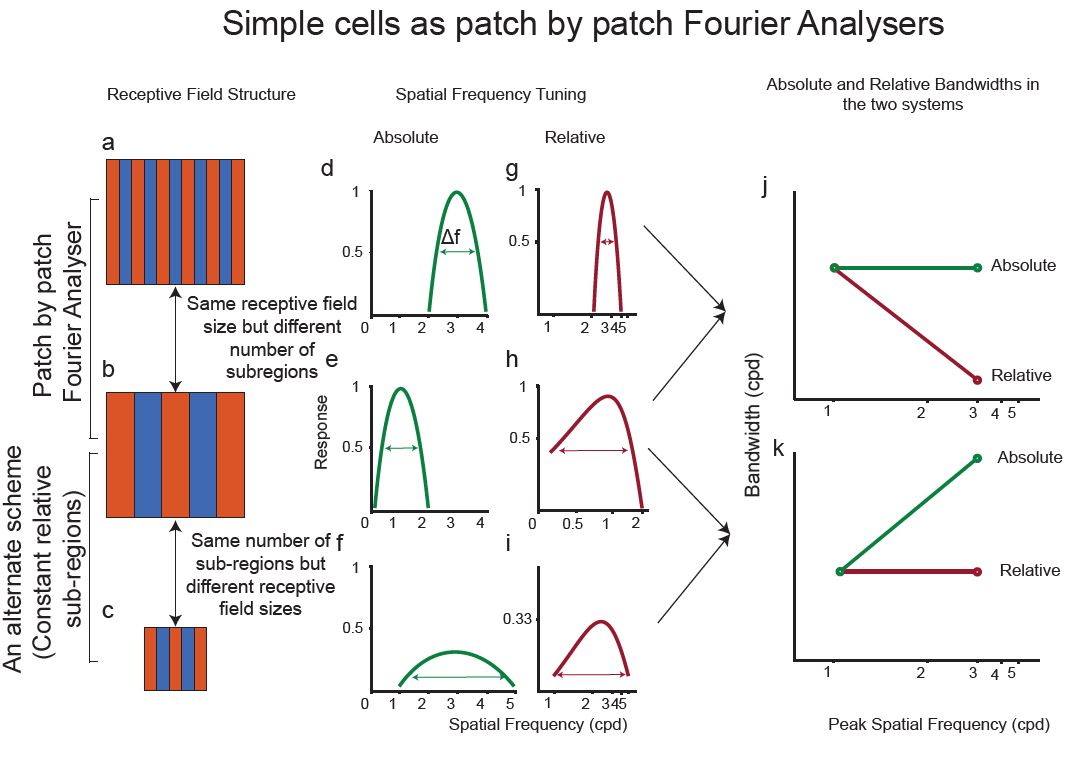
\includegraphics[width=\linewidth]{LinearV1/scheme.jpg}
		\caption{Distribution of segregation indices of neurons.}
		\label{fig:fig1}
	\end{figure}

	As mentioned earlier, neurons in the primary visual cortex can be classified as simple or complex cells. The criteria mentioned by Hubel and Wiesel (1962) are all subjective methods of classifying cells into simple cells. Since then, more objective methods of classifying receptive fields into simple and complex have been established. The first method is by calculating the modulation index (MI). The MI is the ratio between the DC and first harmonic component of the temporal modulation neurons exhibit when shown drifting gratings. This method quantifies the “linearity” of a neurons response based on the assumption that simple cells show linear summation within their receptive field sub-regions. Skottun et al (1991) showed that this method successfully divided neurons into two groups which were roughly the same as simple and complex cells divided using the criteria specified by Hubel and Wiesel (1962).
	While the modulation index measured the linearity of the neurons in cats, in macaques and tree shrews, it tended to overestimate the number of simple cells found. In tree shrews, while over 40\% of neurons could be classified as simple using the modulation index, these neurons did not show the segregation of receptive field sub-regions requisite of simple cells (Van Hooser et al., 2013; Veit et al., 2014). This has also been shown to be the case in macaques (References). 
	Further, it has also been suggested that linearity is not a requisite feature of simple cells. Neurons in the LGN maybe classified as X, Y and W cells. While X cells show linear sustained responses, Y cells exhibit transient, non-linear responses. While originally thought that X and Y cells projected to simple and complex cells respectively, this connection has since been disproved. As a result, significant non-linearities may be introduced in simple cells depending on the type of input that they receive. Further, if simple cells do function as edge detectors rather than linear filters, they are unlikely to be linear neurons (DeValois and Webster, 1978). Hence, alternate methods of classifying simple cells are also examined below. 
	Whether there are cortical simple and complex cells have also been debated. Depending on stimulus parameters, there seems to be a continuum of neurons rather than a bimodal distribution of neurons in the primary visual cortex. So the linear component of all neurons have also been subjected to the same analysis.
	
	\section{Methods}
		
		\subsection{Surgery and Anaesthesia}
		Surgical procedures are as outlined in the Methods chapter. Briefly, the animal was anaesthetized using a mixture of Ketamine and Xylazine, a venous catheter was inserted in to the femoral vein and a tracheostomy performed to assist in breathing during the experiment. The animal was administered muscle paralysant (Vecuronium Bromide) intravenously and was anaesthetised using Isoflurane (0.5-1\%) for the duration of the experiment. Hard contact lenses were fitted to the eye to prevent corneal drying. In some tree shrews, additional lenses were used to correct for any refractive errors. A craniotomy and durotomy were performed over the location of V1 (Horsley-Clarke Co-ordinates A2.5 to P2.5). ECG and frontal EEG were monitored during the experiment. At the end of the experiment, the animal was euthanized using an overdose of pentobarbital sodium and perfused using 0.1M Phosphate Buffer (PB) solution followed by 4\% Paraformaldehyde in 0.1M PB. The brain was removed and stored in sucrose (20-25\%) for histology.
	
		\subsection{Electrophysiology}
		High impedence, lacquer coated tungsten microelectrodes (FHC Metal Microelectrodes Inc., ME, USA; impedance= 12-18 MΩ) were lowered into the brain at an angle perpendicular to the cortical surface. The signal was amplified and filtered (x 10,000 gain, bandpass filtered between 300-3000 Hz, A-M systems) and fed into an audio speaker as well as an analog to digital converter (Cambridge Electronic Design Limited, Cambridge, UK; digitised at 22.5 kHz). Neurons were recorded from Layers 2/3 and Layer 4. Layer 4 could be identified by a characteristic ‘swish’, first for on stimuli and then for off stimuli, in the tree shrews. Where we no longer heard the swish, we concluded that we exited layer 4 and into layer 5. Neurons in layers 5 and 6 were not recorded from. Lesions (6 μA for 6s) were made at the end of each track. The electrode was withdrawn and lesions were made at regular intervals to trace the path of the electrode through the brain. The data was recorded as a spike trace using the spike 2 software (CED, Cambridge, UK). The spikes were templated and the spike timing exported as a text file. Further analysis was performed using custom MATLAB code (The Mathworks Inc, USA).
		\subsection{Stimuli}
		A hand-held projectoscope was used to mark the receptive field boundaries. Using this, the centre of the monitor was aligned with centre of the receptive field prior to stimulus presentation. Stimuli were presented using a BARCO monitor (Frame Refresh Rate= 80 Hz; Reference Calibrator Plus; Barco Video and Communications, Belgium) and generated using Visage (VSG, Cambridge Research Systems, Cambridge, UK) and custom Stimulus Description Language (SDL) scripts. The monitor had a mean luminance of 32.6 cdm-2. While recording, the monitor was placed at a distance of 114 cm from the eye. For each of the different stimuli described below, ten complete stimulus presentations were completed.
				\subsubsection{Bar Stimuli}
				For each neurons, an initial estimate of optimum orientation was obtained using bars, moving bi-directionally across the screen. The background was a uniform gray screen. Depending on the polarity of the neurons, either a bright bar or a dark bar was used (contrast= 100 \%). The bar was usually 8o long (ranging between 4 and 8 degrees) and 0.5o wide (ranging between 0.1 and 1 degree). A total of 18 different orientations were tested and PSTHs (see methods) were made online using the Spike 2 software. The orientation that yielded the highest firing rate was used for further testing.
				After determining optimum orientation, bidirectional, dark and light (decreasing and increasing contrast) bars of the optimum orientation were used to get the response profile of the neurons to opposite polarities (see Fig. 1). 
				\subsubsection{Grating Stimuli}
				For all neurons, once optimum orientation was determined, spatial frequency tuning of the neurons were studied. Drifting sine-wave gratings (TF= 4Hz, Contrast=100\%) of increasing spatial frequencies (between 0 and 2.2 cpd) and in the optimum orientation were presented to neurons. The responses were recorded and stored for further analysis.
				
   		\subsection{Data Analysis}
		Regardless of the stimulus presented, the following analysis was performed on the extracellular trace before any specific analysis was undertaken. Spikes were templated and the spike time and stimulus markers were exported into text files. Using custom scripts in MATLAB, PSTHs (bin-width= 20ms) were constructed for each of the stimulus conditions.  Spike density functions were created using a moving Gaussian envelope with σ of 60 ms (3 bins). This SDF was used for further analysis. 
				\subsubsection{Analysis of Bar Stimuli Responses}
				Orientation tuning was analysed and presented in an earlier chapter. Here is the method by which the dark and light bar data was analysed.
					\paragraph{Calculating Segregation Index (SI)}
					For neurons where dark and light bar data was available, the segregation index (SI) was calculated using the following formula: 
					\[SI=\frac{\sum|R_ton-R_toff|}{\sum|R_ton+R_toff|}\]
					Where, R\_ton is the response of the neuron to a light bar and R\_toff is the response of the neuron to a dark bar (see figure 1). The resulting value was a number between 0 and 1. Neurons with high segregation index (>0.5) were more likely to have segregated dark and light sub-regions and were hence categorised as simple cells. Likewise, neurons with low segregation indices were classified as complex cells as they were less likely to have segregated dark and light sub-regions.
				
				\subsubsection{Analysis if Grating Stimuli Responses}
				
				For all neurons, a discrete fourier transform was applied to the PSTH using the MATLAB fast fourier transform algorithm (FFT). The DC (F0) and the first harmonic component (F1) of the response was used for further analysis. Optimum spatial frequency for the neurons was determined as explained in Chapter 4. The modulation ratio was then calculated as follows.
				
				\[Modulation Index (MI)= 2*\frac{F_1}{(F_1+F_0)}\]
				
				Where Rf1 and Rf0 are the responses of the F0 and F1 components at the peak spatial frequency.
				The modulation ratio returned a number between 0 and 2. If the neuron had a modulation index greater than 1, it was classified as simple and it was classified as complex otherwise (Van Hooser et al., 2013). Only neurons classified as simple cells were used for further analysis and only the F1 component of the responses were further analysed.
				For each neuron, two spatial frequency tuning bandwidths were calculated. One was the absolute bandwidth which was the difference between the upper and lower cutoff spatial frequencies. The upper cut off was calculated as the spatial frequency greater than the peak spatial frequency where the response first reaches half the maximum response. The lower cutoff was calculated similarly for spatial frequencies lower than peak spatial frequency where response first reached half the maximum response. If the response never reached half the maximum response, the neuron was classified as low pass or high pass tuned. The relative bandwidth was then calculated as the absolute bandwidth/ peak spatial frequency.
				
		\subsection{Histology}
				The brains were stained for Nissl substances using cresyl violet acetate and lesions were located. The number of neurons found in each layer have been presented in V1 chapter and are not presented here. However, for all the results presented here, layer specific results are also presented.
							
					

	\section{Results}
	
		Results from a total of 64 neurons are presented below. Where possible, the layerwise distribution is also presented. 
		
	\paragraph {Segregation Index}	
	In 49 of the 64 neurons, we recorded the response of the neuron to dark and light bars. Simple cells have segregated receptive fields which appear as separate peaks in the PSTHs (Fig 1a) and complex cells have overlapping subregions which appear as overlapping peaks in the PSTH (Fig 1b). Accordingly, the segregation index is higher for simple cells compared to complex cells.
	
		\begin{figure}[H]
		
		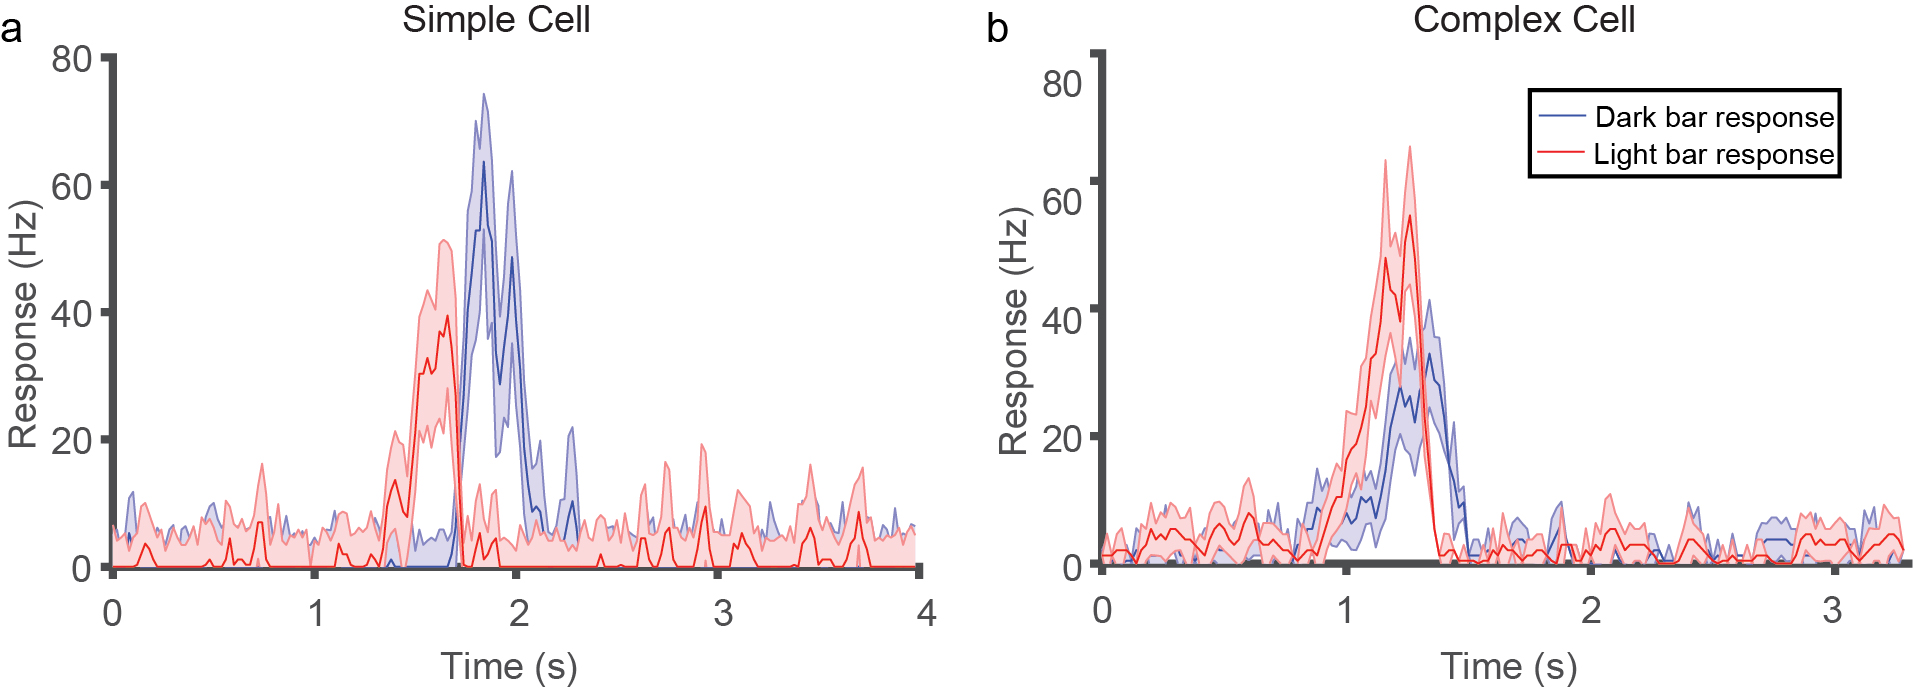
\includegraphics[width=\linewidth]{LinearV1/simplecomplex.jpg}
		\caption{Response of a simple (a) and complex cell (b) to the dark and light bar stimuli. The spatially segregated RF of the simple cells is translated into the temporally segregated response of the neuron. Whereas, in the complex cell, the overlapping sub-regions are reflected in the temporally overlapping response of the neuron. Accordingly, the simple cell has a high SI (0.92) and the complex cell has a lower SI (0.39).}
		\label{fig:fig2}
	\end{figure}
	
	The distribution of segregation index for 47 neurons is presented below. Of the 49 neurons, 19 were from layer 2/3, 12 were from layer 3c and 18 were from layer 4. There was no significant difference in SI between the layers (Kruskal-Wallis test, p=0.34).
	\begin{figure}[H]
		
		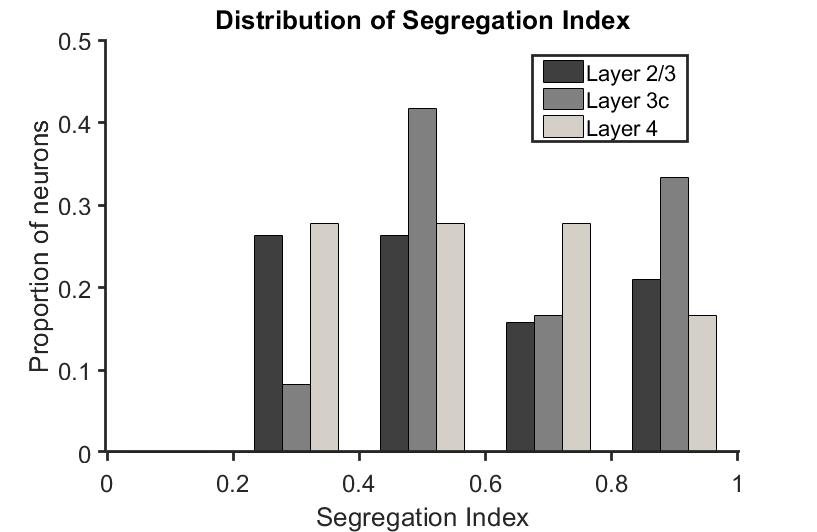
\includegraphics[width=\linewidth]{LinearV1/segregationindex_colouradj.jpg}
		\caption{Distribution of segregation indices of neurons.}
		\label{fig:fig3}
	\end{figure}

	\paragraph{Modulation Index}
	The modulation indices of all the 69 neurons [Layer 2/3= 27; Layer 4= 27; Layer 3c= 15] are shown in figure 3. There was no significant difference in the modulation index between the layers (Kruskal-Wallis test, p= 0.74).
	
		\begin{figure}[H]
		
		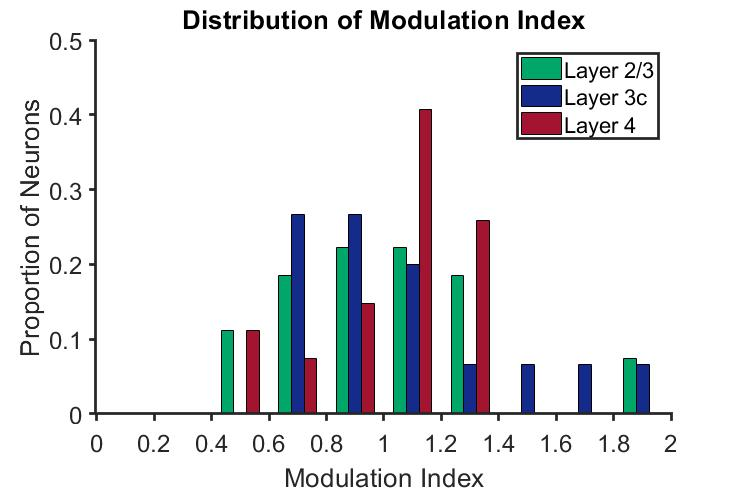
\includegraphics[width=\linewidth]{LinearV1/modind_layer_colour.jpg}
		\caption{Distribution of modulation indices of neurons.}
		\label{fig:fig4}
	\end{figure}
	In neurons where both the segregation index and modulation index were recorded, they were plotted against each other. There was no significant correlation between the two indices (rho=0.02, p=0.89). 
	
	
	\begin{figure}[H]
		
		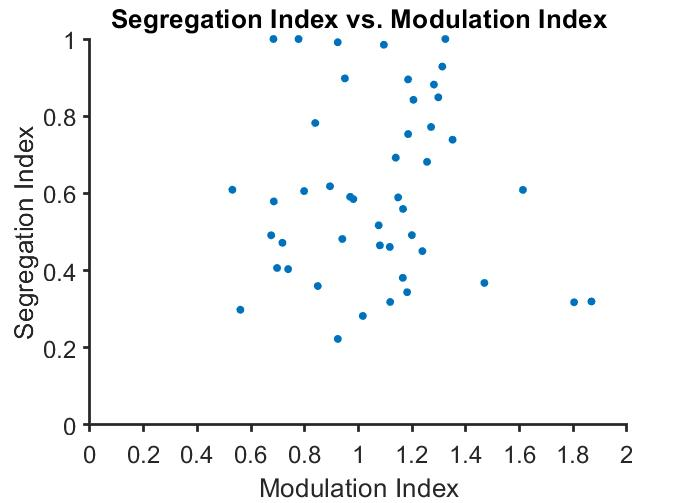
\includegraphics[width=\linewidth]{LinearV1/Segindvsmodind.jpg}
		\caption{Relationship between the modulation and segregation indices.}
		\label{fig:fig5}
	\end{figure}

	\paragraph{Relationship between bandwidth and spatial frequency}
	
	Neurons were classified as simple cells using the modulation index (MI>1), the segregation index (SI>0.5), both the modulation and segregation index together (MI > 1 and SI >0.5). The relationship between the absolute bandwidth and the peak spatial frequency for simple cells classifies as described as above as well as for all the neurons in the sample are shown in figure 5(a,c,,e \& g). Statistically significant relationships are indicated using $*$. For the other two measure used for classification, the correlation was not significant. There was a significant correlation between the when all neurons were used for the analysis. The relationship between relative bandwidth and the peak spatial frequency are shown in the right hand panel. In all cases except for the one in (f) the results were statistically significant.
	
		\begin{figure}[H]
		
		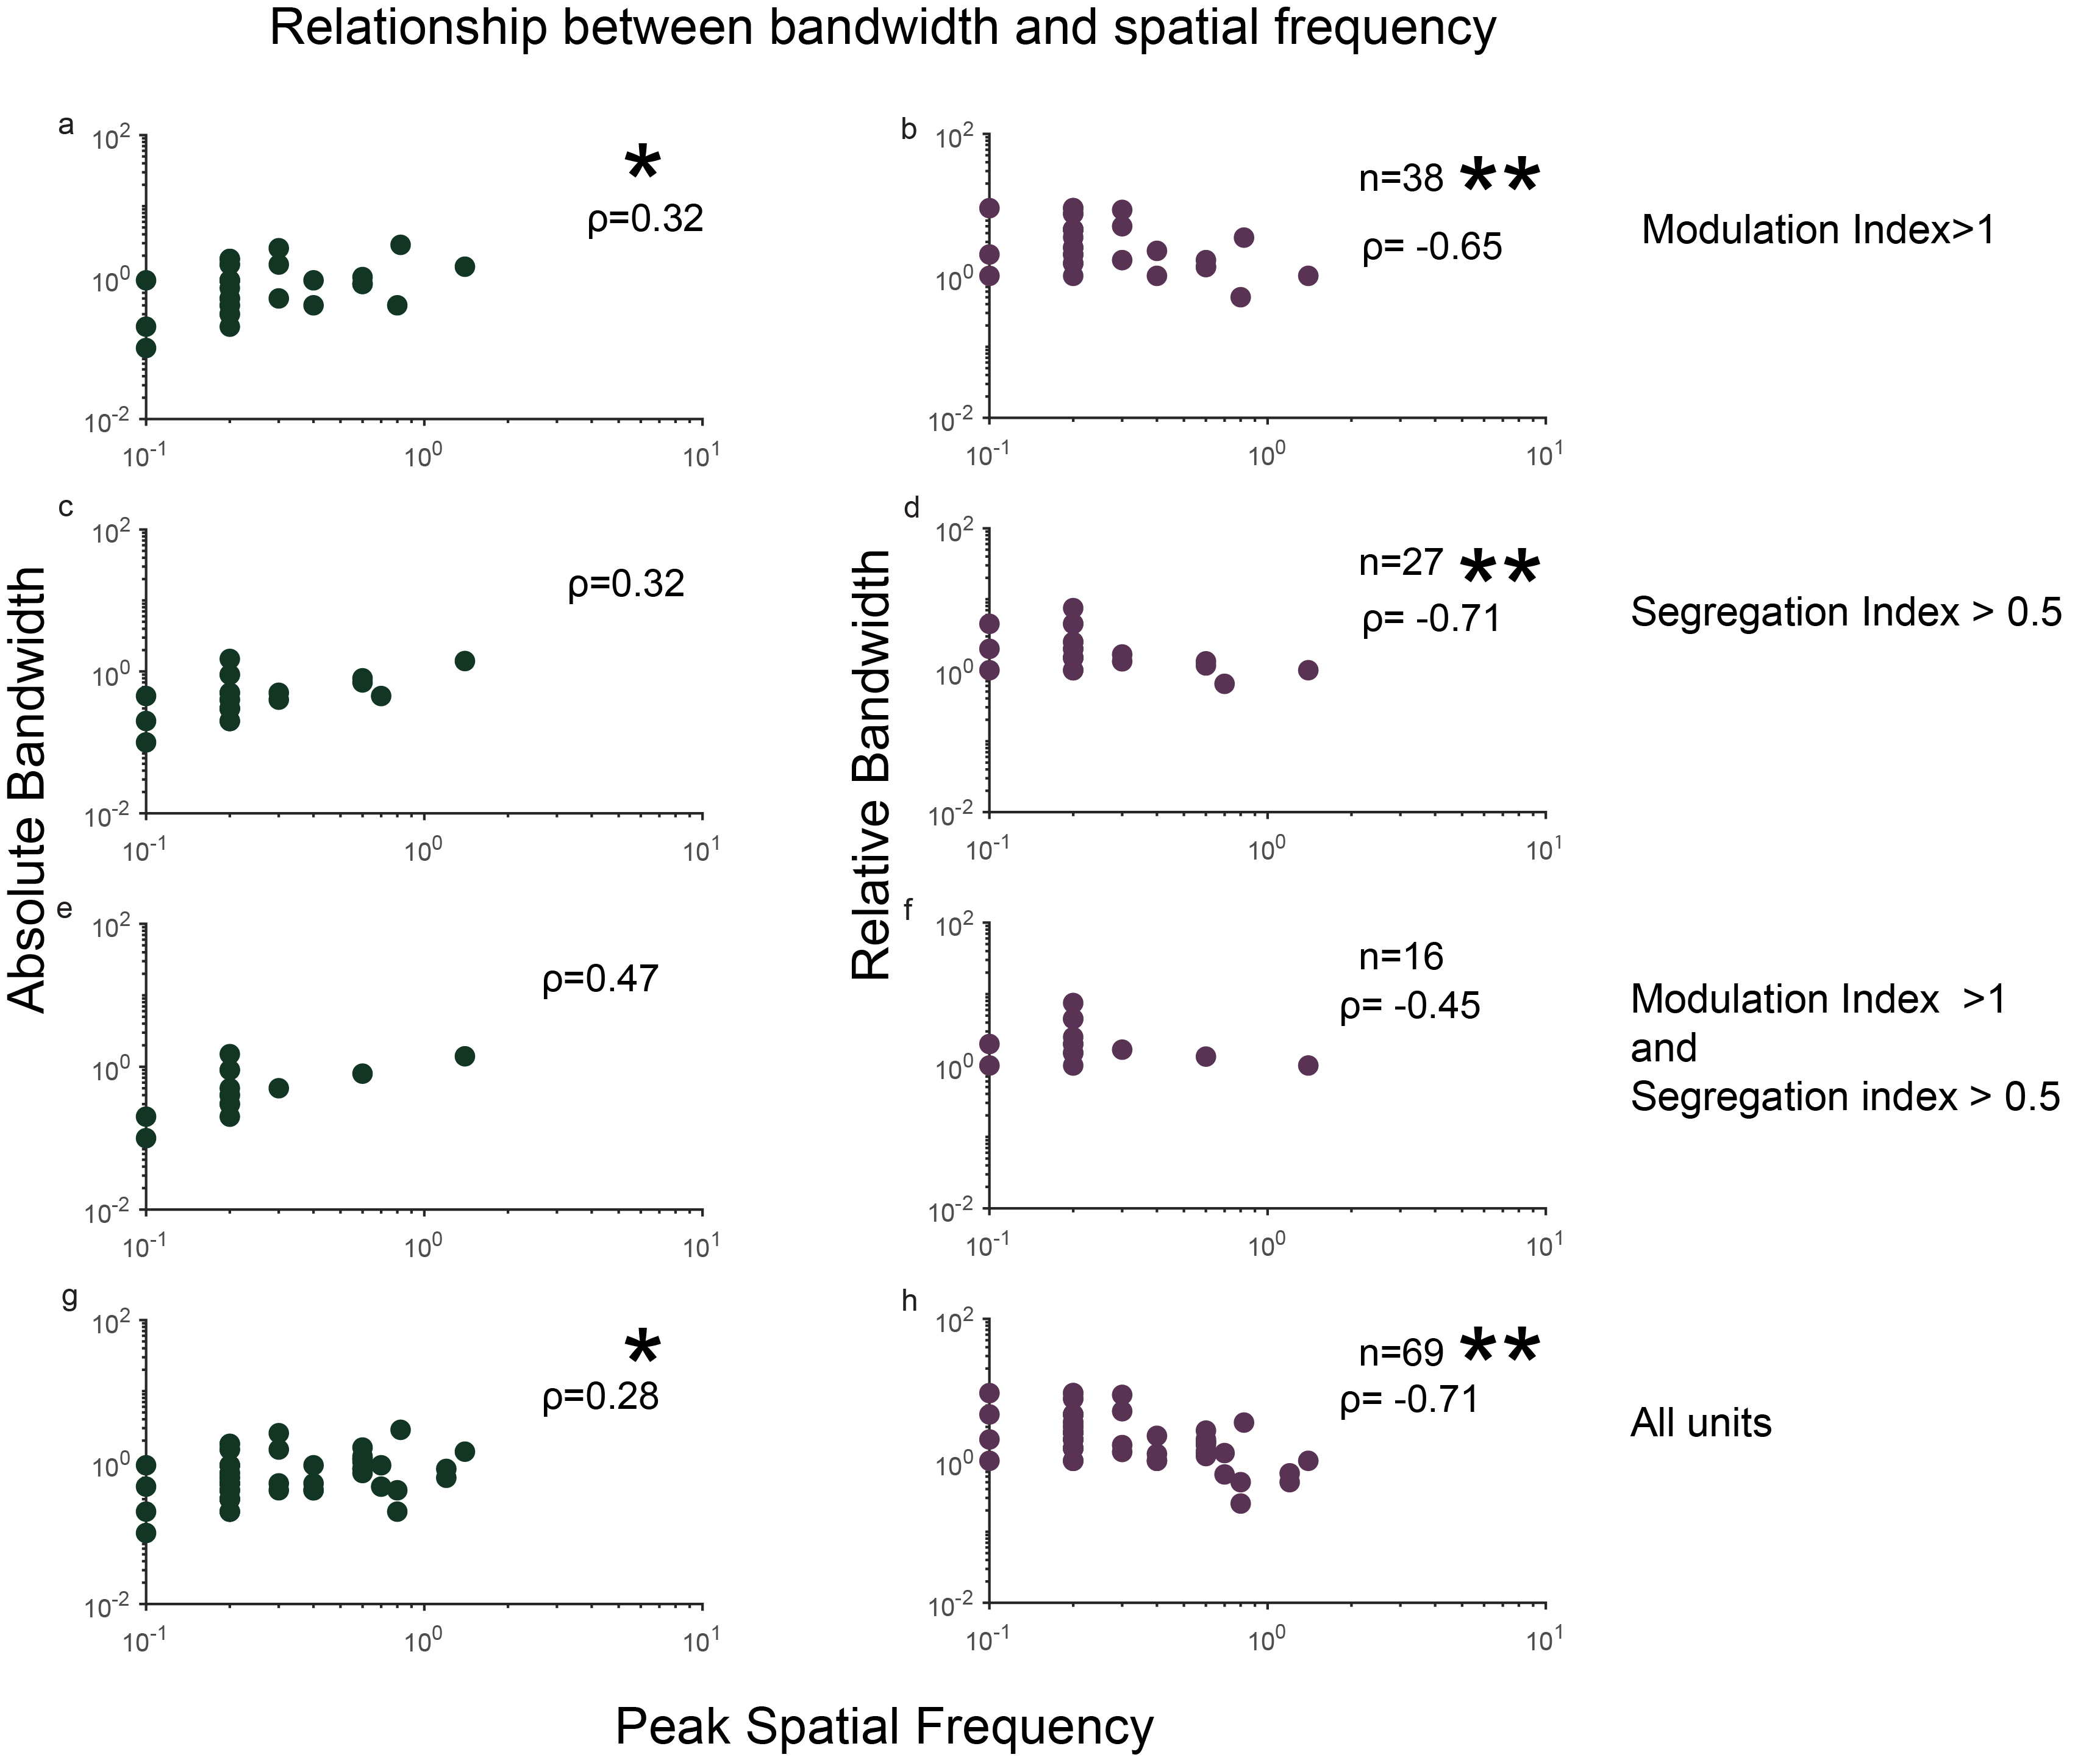
\includegraphics[width=\linewidth]{LinearV1/hwpksf.jpg}
		\caption{This figure shows the relationship between bandwidth and spatial frequency in simple cells when using the modulation index to classify units (a,b), when using the segregation index (c,d); using both the modulation and segregation index (e,f) and for all neurons in the sample (g,h). The plots on the left hand side show the relationship between absolute bandwidth and the peak spatial frequency while the plots on the right hand side show the relationship between the relative bandwidth and peak spatial frequency. Number of units used for generating each plot is specified in the right hand corner and statistically significant results are shown by *. *= p$<$0.05. **=p$<$0.0001.}
		\label{fig:fig6}
	\end{figure}
	
	
	\section{Discussion}
	
	In this chapter, we investigated whether neurons in the tree shrew V1 behaved like patch by patch Fourier analysers. Our results show while most simple cells do not behave like ideal Fourier analysers, they are still far better Fourier analysers than the neurons in cat and macaque striate cortex.
	
	In order to classify the neurons into simple and complex cells, we used two objective measures that are regularly used in the literature: a) The Segregation Index and b) The Modulation Index. The SI measures the degree of separateness of the receptive field sub-regions i.e., if there are separate on and off sub-regions. Using this measure, we found that about half the neurons for which this data was available for were simple. The MI on the other hand measures the degree of linear summation over the receptive fields. Using this measure too, a similar proportion of  neurons were classified as simple cells. However, there was no significant correlation between the two measures (See fig.\ref{fig:fig5}). This indicates that different neurons are classified as simple based on the two different measures. Only half the neurons that were classifies as simple using the SI were also classified as simple using the modulation index, indicating that atleast half the neurons that show linear summation over their receptive field also had overlapping sub-regions. 
	
	Of the neurons that were classified as simple using both MI and SI, there was no statistically significant correlation between the peak spatial frequency and the absolute bandwidth. However, this doesn't necessarily mean that these neurons do not function as Fourier analysers. A power analysis showed that for an expected correlation of -0.45, the sample size had to be atleast 36 for a statistically significant result. It could simply mean that there was not enough neurons in our sample.
	
	The distribution of SI and MI in our results show that neither of these values differ significantly across layers. The SI seems to be distributed almost uniformly across the whole range of possible values (between 0 and 1). However, it is interesting to note that no neurons showed complete and equally overlapping subregions (SI $<$ 0.2; see fig.\ref{fig:fig3}). These results are also consistent with those published by Van Hooser et al., 2013 (see fig 3c). This could mean that most neurons in the shrew V1 receive unbalanced on and off inputs. (Check Bimodality Index). Previous studies have suggested that the tree shrew V1 has a preponderance of off dominated neurons. It has also been suggested that this off dominance could be the origin of orientation selectivity in the V1 of tree shrews. Another reason for the difference could also be the way SI is calculated. The SI is calculated from the temporal profile of the neuronal response to light and dark bars. While this gives an accurate enough measure, it may not be sensitive enough to detect small differences in sensitivities between the off and on regions.
	
	While the distribution of MI was not significantly different between the layers, there are a few important trends that may be of note. First, while the layer 2/3 and layer 3/c distribution look identical, a majority of Layer 4 neurons seem to have a modulation index greater than 1 (see fig.\ref{fig:fig4}). This is consistent with reports in literature where the simple cells are present predominantly layer 4 with some complex cells also found in this layer. However, a significant proportion of layer 2/3 and layer 3c neurons are also highly modulated, simple like neurons, which are reported only rarely in the literature (References). 
	
	Here we used a modified version of the modulation ratio (F1/F0) to quantify the degree of linear summation within the receptive field. In the original modulation ratio, neurons were only classified as simple if their F1/F0 ratio was greater than 1.57 (Skottun et al., 1991; Movshon et al., 1978). This number roughly translates to an MI of 1.2. Therefore, while neurons whose MI are between 1 and 1.2 have a greater modulated component of the response compared to the unmodulated component, they still show significant non-linearities. These neurons have been classified previously as 'b' cells. In our sample, we also found that these neurons were dominated by one polarity (either on or off), which also makes sense as on and off neurons are segregated into layers in the shrew V1.

	Finally, the distribution of SI and MI observed in our data also calls into question the age old question of whether simple and complex cells are two separate categories of neurons or if they lie on a continuum. Our data shows that both these measures are unimodally distributed and not bimodally distributed in line with previous studies which have suggested a similar pattern. Further, it has also been suggested that under certain circumstances, simple could behave like complex cells and complex cells could behave like simple cells. This property of neurons has been implicated in their ability to transmit signals; i.e., simple cells will behave like simple cells when their output is relevant for perception but not otherwise.

	Plan:
	1) Summary of results
		Differences in modulation index and segregation index. What this means? Linearity of neurons?
		Segregation index: no neurons that had completely overlapped sub-regions i.e. si<0.2.
		with the rest of the SI, evenly distributed across the layers.
		There was no significant differences between layers.

		Modulation index: Although not statistically significant, modulation index<1 for most layer 2/3 and layer 3c. modulation index>1. Most layer 4 neurons, have a modulation index between 1 and 1.2. This is the equivalent of between 1 and 1.57 using the standard modulation ratio calculated (F1/F0). These neurons still have a higher modulation index but not high enough. Could be potential B cells described by Henry et al or the non-linear simple cells described by other people. 
		
		Simple cells are found in input layers while complex cells are found in supragranular layers. True if we look at the modulation index but not when looking at the segregation index. Provides support against the heirarchical model of visual processing where simple cells project to complex cells. Also has been shown in other species- complex cells are found in layer 4 and simple cells in supragranular layers. We see the same trend here.
		
		How do our results of segregation index and modulation index compare with the previously published results for segregation and modulation ratios?  Our results are similar to previously published results by Van Hooser et al., 2013. Both results seem to show a unimodal distribution with a range of linearities in the receptive fields when compared to a simple/complex bimodal distribution. Is this because of the measure used for modulation index? Checked with regular modulation index (F1/F0) This measure also did not yield a bimodal distributions.
		
		What does the relative bandwdth and spatial frequency relationship mean?
		
		We found that in most cases, there was a negative relationship between the pk spatial frequency and the relative bandwidth of the neurons, especially when the linear component of all the neurons were used to run the analysis. This means that most neurons in the shrew V1 actually do act as linear filters in optimum range of the neurons (See Fig.\ref{fig:fig1}).
		What exactly does this mean? The cortex could be completely throwing out this information when non-linear?
		
		What is linearity even useful for?
		ARe there simple and complex cells in the shrew cortex? Does this mean anything?